% This is samplepaper.tex, a sample chapter demonstrating the
% LLNCS macro package for Springer Computer Science proceedings;
% Version 2.20 of 2017/10/04
%
\documentclass[runningheads]{llncs}
%
\usepackage{graphicx}
% Used for displaying a sample figure. If possible, figure files should
% be included in EPS format.
%
% If you use the hyperref package, please uncomment the following line
% to display URLs in blue roman font according to Springer's eBook style:
% \renewcommand\UrlFont{\color{blue}\rmfamily}

\begin{document}
%
\title{Poshet}
%
%\titlerunning{Abbreviated paper title}
% If the paper title is too long for the running head, you can set
% an abbreviated paper title here
%
\author{Sabina-Alina Prodan}
%
\authorrunning{S. Prodan}
% First names are abbreviated in the running head.
% If there are more than two authors, 'et al.' is used.
%
\institute{Universitatea "Alexandru Ioan Cuza", Iași, România}
%
\maketitle              % typeset the header of the contribution
%
\begin{abstract}
Poshet este un client pentru serviciul POP3 în care se poate vizualiza, organiza și trimite e-mail. În continuare sunt detaliate atât tehnologiile utilizate, structura aplicației, cât și diverse detalii de implementare.

\keywords{C++ \and Email \and POP3 \and SMTP \and MIME \and wxWidgets}
\end{abstract}
%
%
%
\section{Introducere}

Poshet este un client cu interfață grafică, scris în C++ cu wxWidgets, pentru serviciile de mail electronic POP3 (pentru obținerea de mailuri) și SMTP (pentru trimiterea de mailuri). Printre funcționalitățile acestuia se numără: vizualizarea și organizarea mailurilor primite, trimiterea de mailuri noi cu atașamente, reply sau forwarding la mailuri primite.

\section{Tehnologii aplicate}

Proiectul este scris în C++ utilizând OOP. Pentru compilarea sa sunt folosite atât fișiere \texttt{Makefile}, cât și CMake. Proiectul include un fișier \texttt{README.md} care detaliază procesul de compilare.

Comunicarea în rețea cu serverele POP3 și SMTP se realizează prin intermediul funcțiilor POSIX. Protocolul ales la nivel de transport este TCP, fiindcă ambele protocoale la nivel de aplicație sunt bazate pe acesta.

Comunicarea cu baza de date SQLite creată local se realizează cu ajutorul librăriei SQLite3. În comparație cu alternative precum XML, o bază de date concretă permite interogări mai complexe și o organizare mai ușoară a mailurilor dintr-un inbox.

Pentru interfața grafică este utilizată librăria wxWidgets (în pofida altor librării similare precum Qt) datorită simplității sale, a structurii bazate pe OOP și în mod special a integrării sale facile cu Visual Studio Code și CMake.

Pentru analizarea și procesarea mailurilor din conținut ASCII într-un format afișabil în client se utilizează o librărie externă (Mimetic) pentru fișiere scrise conform standardului MIME\cite{ref_rfc_mime}. A fost aleasă o librărie externă pentru că standardul MIME este destul de complex și se dorește o soluție implementată cât se poate de corect și testată riguros.



\section{Structura aplicației}


\subsection{Arhitectura principală}

Proiectul folosește clase și OOP, având o structură inspirată în linii mari de arhitectura MVP (Model-View-Presenter) pentru a separa responsabilitățile între clase.



\subsection{Detalii despre clasele programului}


Principala clasă care face legătura între interfețele aplicației și logica din spate (comunicarea cu servere, cu baza de date, etc.) este AppController. Aceasta administrează și comunică cu instanțe ale interfețelor LoginFrame, DashboardFrame și MailCreatorFrame și o instanță a clasei Session.

Session este clasa care se ocupă de comunicarea cu resurse externe pentru a obține și furniza informații. Aceasta solicită și trimite informații către instanțe ale altor clase specializate, care realizează operații precum obținerea mailurilor noi, salvarea lor în baza de date, trimiterea unui mail nou, sau salvarea locală a unui atașament.

În momentul primirii de notificări de la interfețele la care AppController este "abonat", AppController se ocupă de interacțiunea cu clasa Session pentru a obține informații și a le transmite către interfețe, care trebuie să folosească datele pentru a se actualiza și a le afișa către utilizator.

Clasa AppController poate fi privită ca un mediator între interfețe și logica programului, interacționând cât mai puțin cu librăria grafică și nefiind implicat în comunicarea efectivă în rețea.


\subsection{Stocarea informațiilor}

Datele care aparțin unui mail sunt păstrate cu ajutorul clasei Mail, care conține metode prin care se poate procesa conținutul unui buffer ASCII (scris conform standardului MIME) și se pot obține informații precum headers, date plain-text, atașamente, etc. În momentul când se dorește afișarea conținutului unui mail pe ecran, interfața DashboardFrame este responsabilă cu afișarea datelor mailului în viewMailPanel, utilizând elemente specializate ale wxWidgets precum wxRichTextCtrl (care permite afișarea "inline" de imagini sau alte fișiere multimedia).

De asemenea, mailurile primite sunt stocate într-o bază de date locală, într-o tabelă \texttt{Mail} (legată de tabela \texttt{Users} printr-o relație de tip "one-to-many"). Pe lângă datele "raw" ale mailurilor sunt stocate și informații adiționale precum headers importante (To, Subject, etc.) sau un "tag" prin care utilizatorul a marcat respectivul mail în client pentru a își organiza inboxul.


\begin{figure}
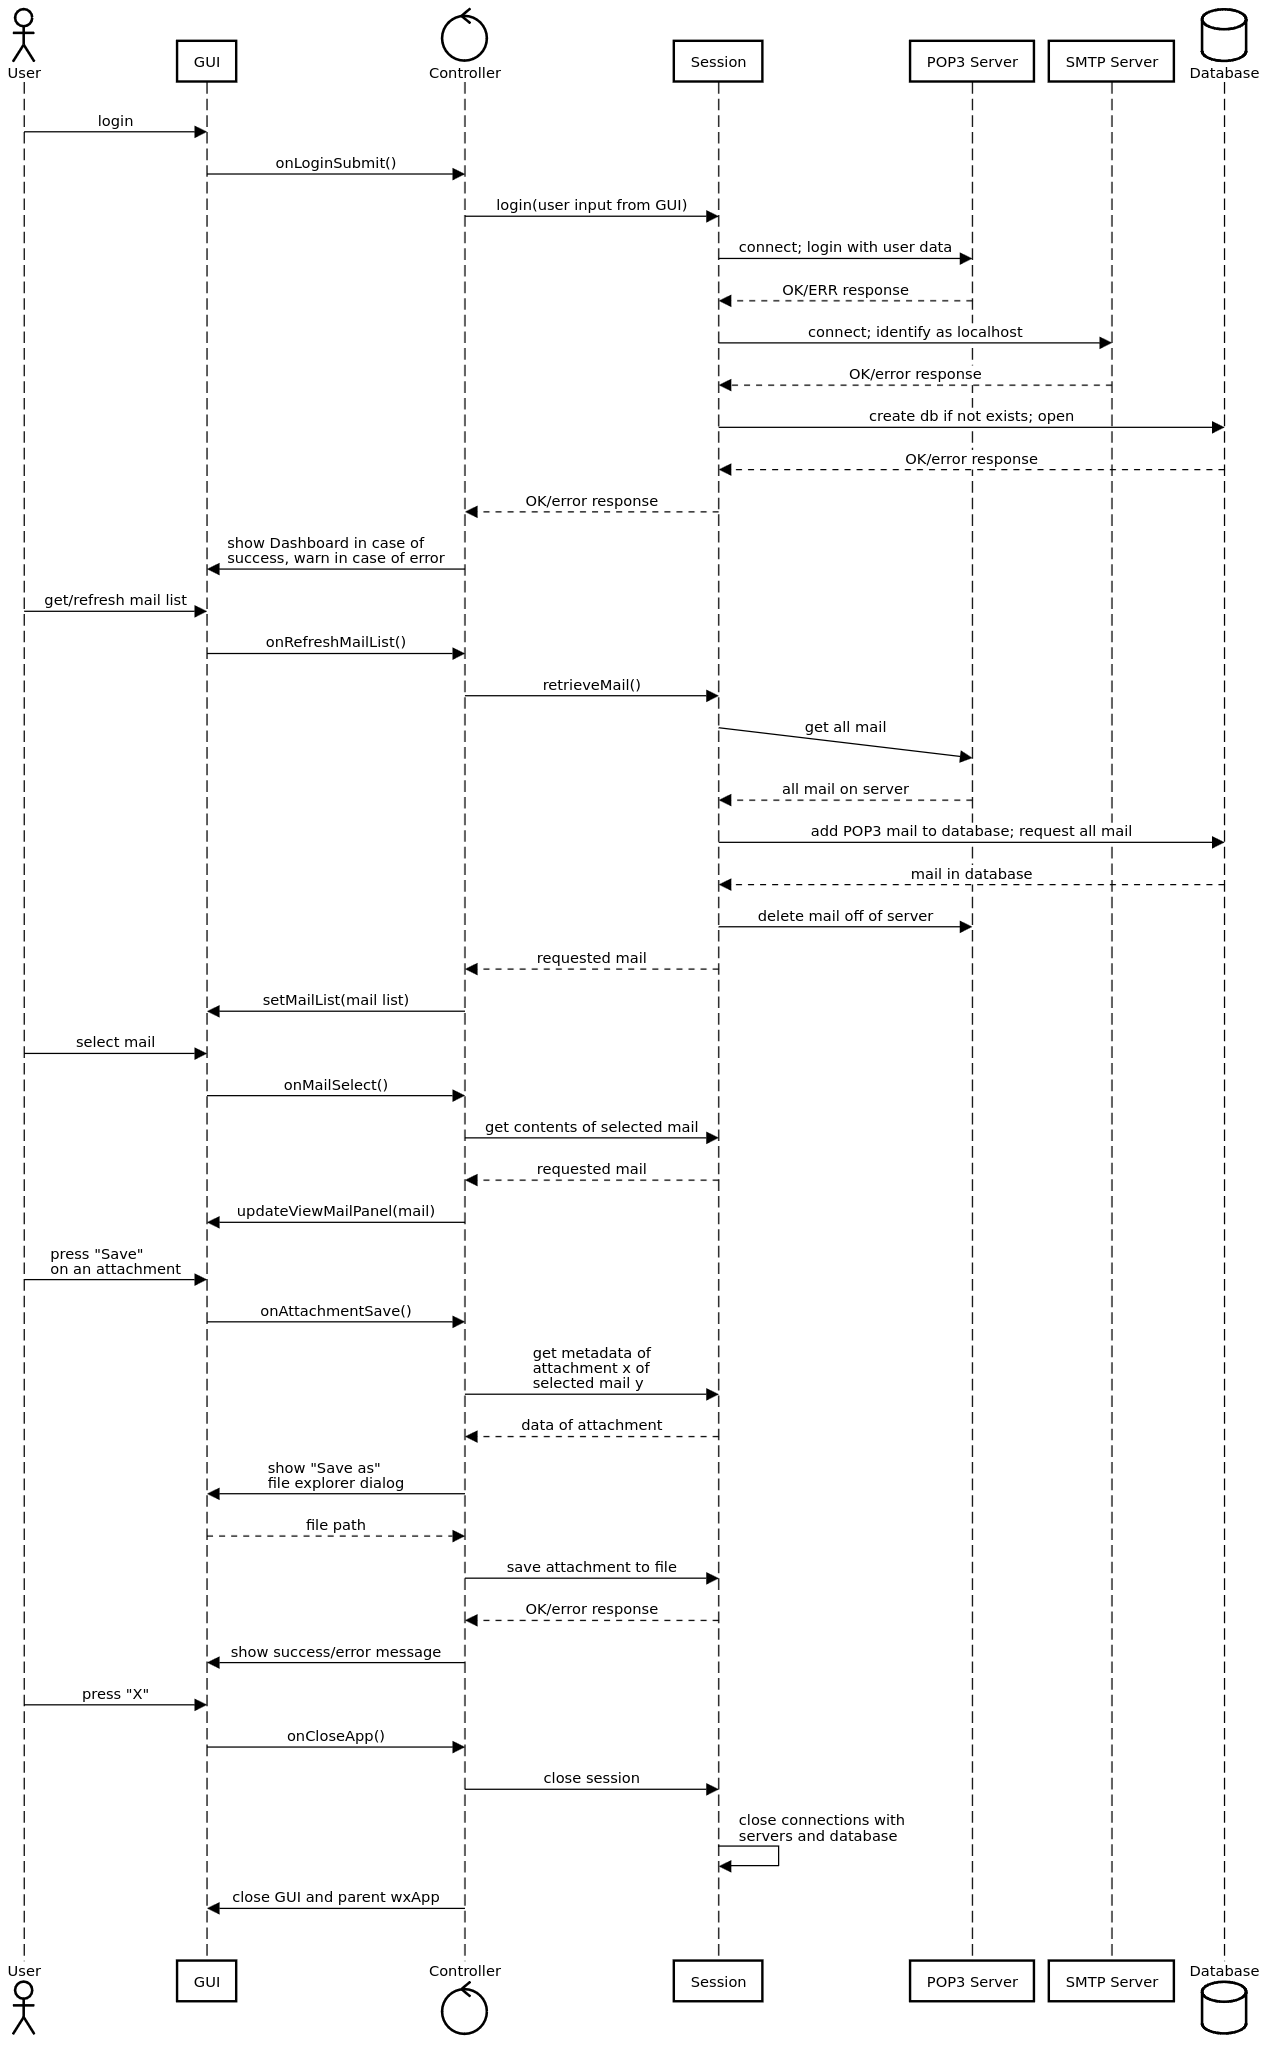
\includegraphics[width=\textwidth]{halfDiagram1.png}
\caption{Diagrama secvențială a aplicației, partea 1: aici sunt ilustrate mecanismele de logare, afișare a mailurilor primite, și închidere a aplicației.} \label{firsthalf}
\end{figure}

\begin{figure}
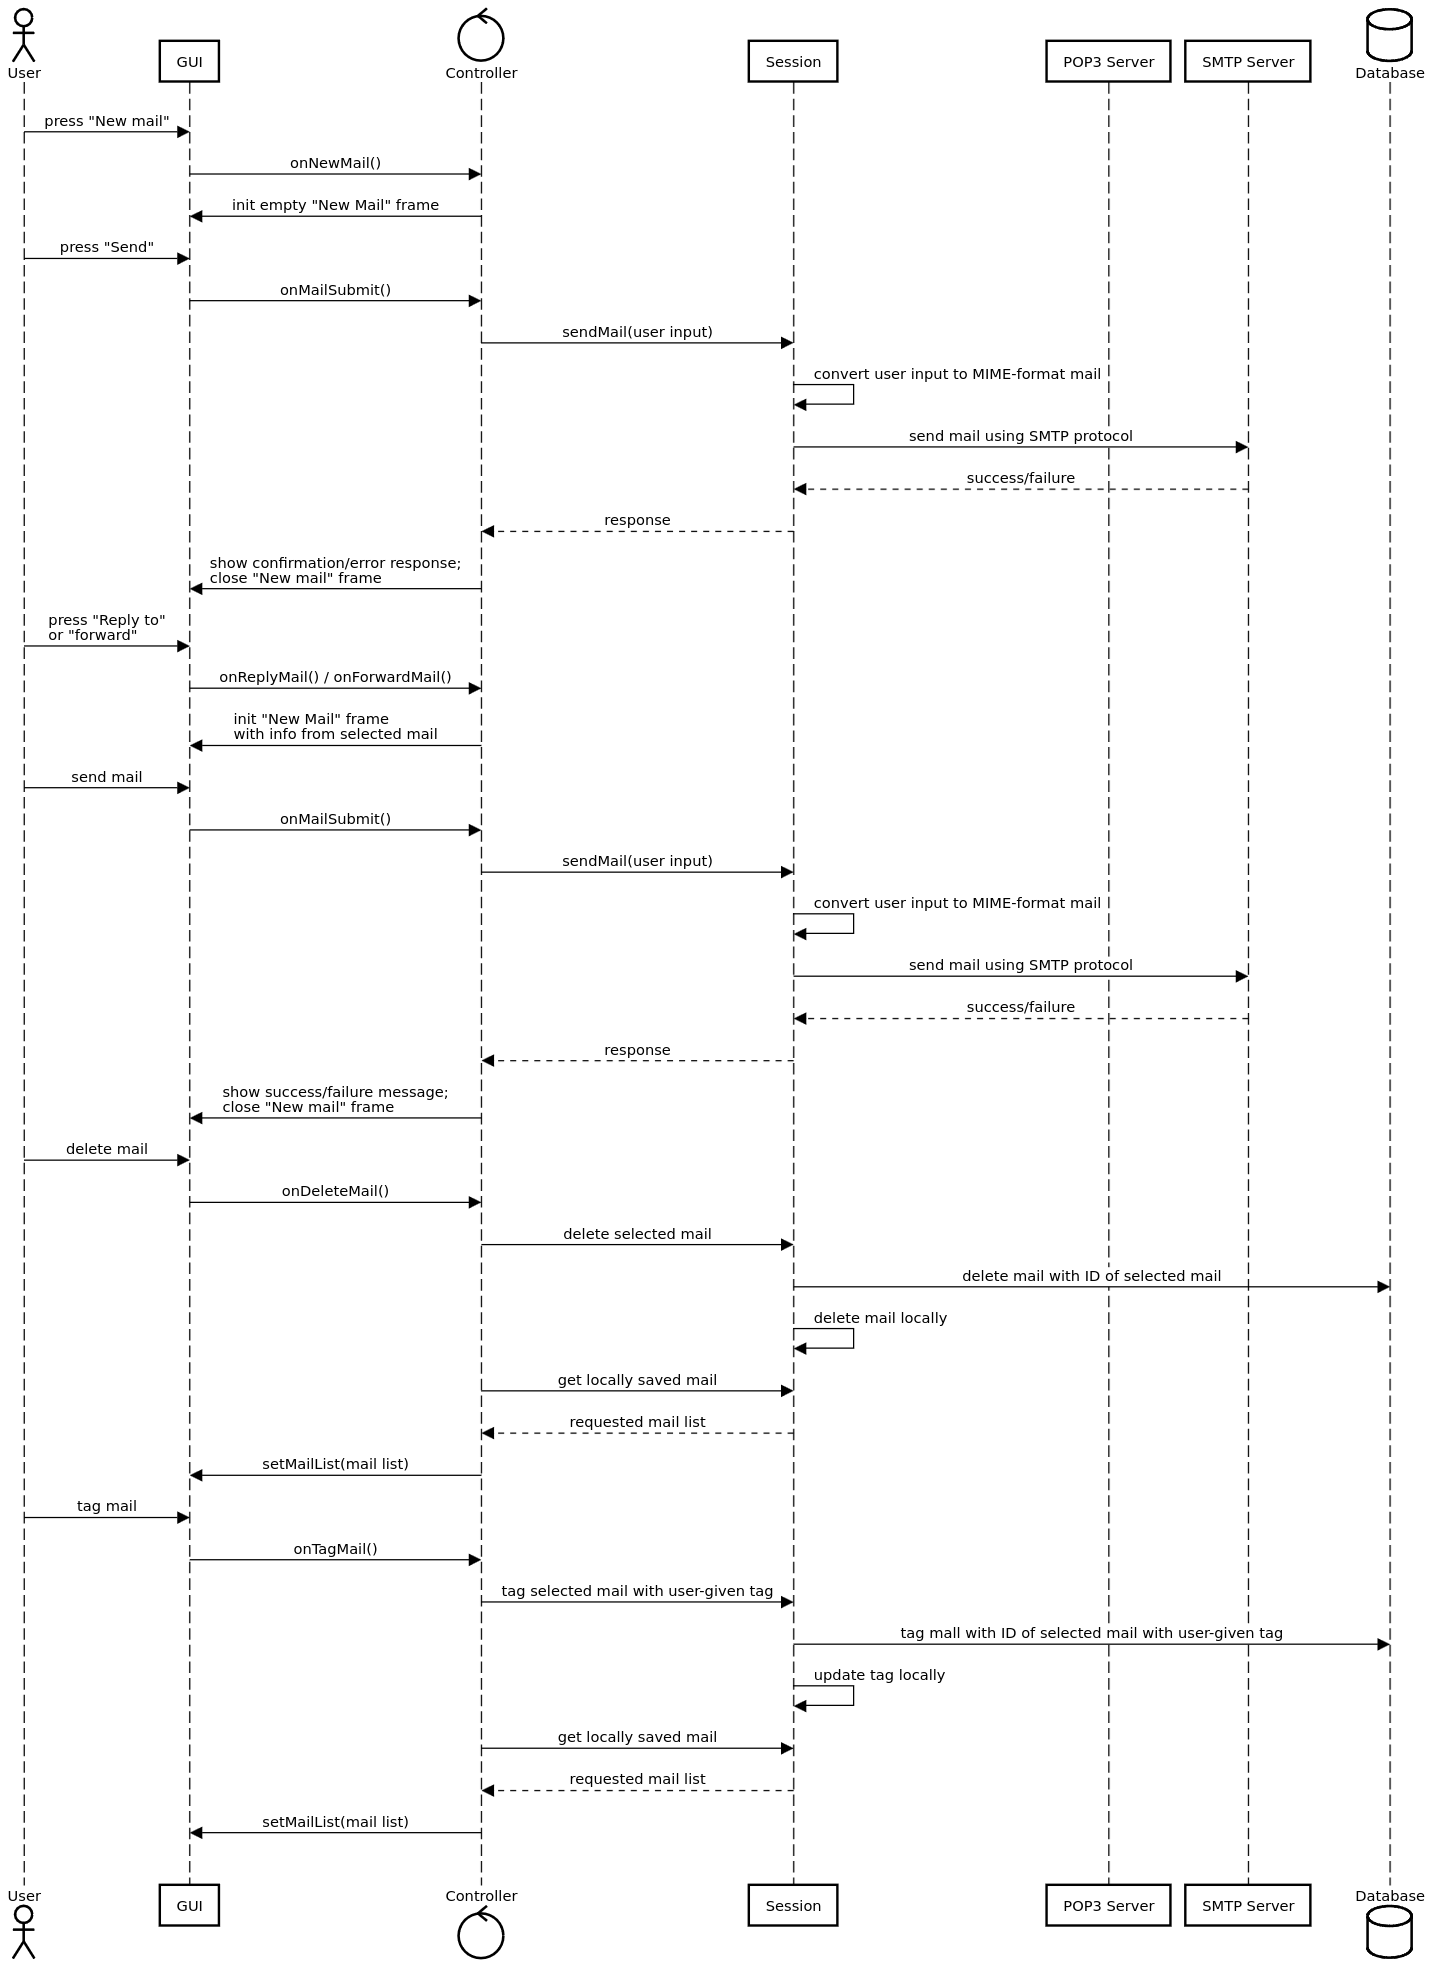
\includegraphics[width=\textwidth]{halfDiagram2.png}
\caption{Diagrama secvențială a aplicației, partea 2: aici sunt ilustrate mecanismele de trimitere de mail nou și organizare de mail primit.} \label{secondhalf}
\end{figure}


\newpage




\section{Aspecte de implementare}

\subsection{Protocoale utilizate}
Proiectul constă într-un client pentru servere existente, deci acesta se folosește de protocoale la nivel de aplicație deja existente.

Pentru obținerea mailurilor se folosește protocolul POP3\cite{ref_rfc_pop3}, iar pentru trimiterea de mailuri se folosește protocolul SMTP\cite{ref_rfc_smtp}. Clasele responsabile de conexiunile POP3 și SMTP trimit comenzi corespunzătoare funcționalităților dorite de utilizator, recunoscute de servere; spre exemplu, \texttt{USER} / \texttt{PASS} pentru autentificare POP3, \texttt{RETR} pentru lista de mailuri, \texttt{LIST} pentru datele unui mail particular, \texttt{MAIL TO} și altele pentru trimiterea unui mail, etc.

Ambele protocoale sunt de tip comandă-răspuns; așadar, în urma trimiterii comenzii se așteaptă răspuns afirmativ (sau un mesaj de eroare) de la server, informația fiind apoi transmisă la funcțiile care au solicitat-o.

\subsection{Scenarii de utilizare}
Poshet este menit să comunice cu un server POP3 ne-încriptat, cu autentificare plain-text, și cu un server SMTP fără autentificare. În timpul dezvoltării acestui proiect s-au folosit programele Dovecot și Postfix pentru a configura servere POP3 și respectiv SMTP pe \texttt{localhost}.

Un client de acest tip poate fi folositor în situații precum testarea locală; unele procese pot fi configurate să trimită mail către serverul SMTP local (spre exemplu, pentru a simula trimiterea de mail către mai mulți utilizatori ai unui serviciu), iar administratorul le poate citi, verifica și organiza ușor din aplicație. De asemenea, prin conectarea la serverul SMTP local cu acest client se poate testa și verifica funcționarea conformă a serverului.

\subsection{Aspecte interesante legate de implementare}

\subsubsection{Utilizarea sistemului de "subscribers".} Pentru a evita dependența circulară între clasa AppController și clasele de interfață, dar și pentru a minimiza interacțiunea cu AppController prin modalități specifice librăriei wxWidgets, se utilizează conceptul de "subscribers".

AppController implementează simultan trei clase pur virtuale: LoginFrameSubscriber, DashboardFrameSubscriber și MailCreatorFrameSubscriber. În momentul creerii LoginFrame, DashboardFrame și respectiv MailCreatorFrame, AppController apelează metodele publice \texttt{subscribe} ale acestora, iar fiecare instanță de interfață memorează o referință la AppController sub forma unui pointer de tipul "subscriber" corespunzător. Fiindcă interfețele în sine sunt administrate de către AppController, nu există riscul ca una dintre interfețe să apeleze o metodă în timp ce "subscriber"-ul său să fie un pointer invalid.


\begin{figure}
    \centering
    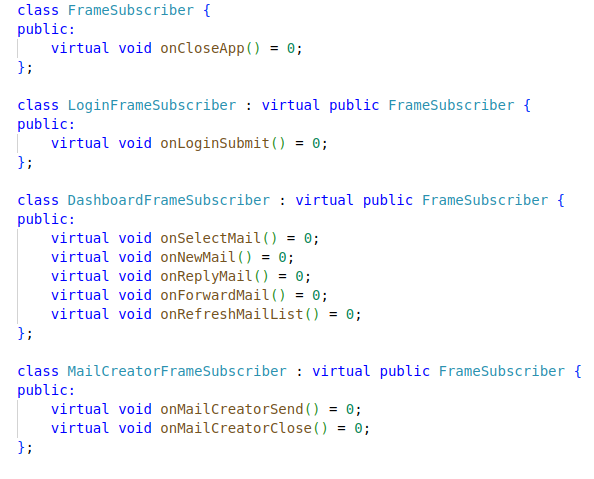
\includegraphics[width=\textwidth]{subscribers.png}
    \caption{Declararea claselor pur-virtuale de tip "subscriber" în \texttt{FrameSubscribers.hpp}.}
    \label{fig:subscribers}
\end{figure}


\begin{figure}
    \centering
    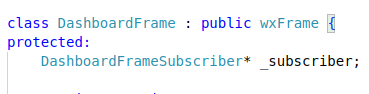
\includegraphics[width={200px}]{subscriberMember.png}
    \caption{Definirea membrului \texttt{\_subscriber} în \texttt{DashboardFrame.hpp}.}
    \label{fig:subscriberMember}
\end{figure}

\newpage

În wxWidgets, interacțiunea utilizatorului cu o interfață este semnalată acesteia prin intermediul unor \texttt{wxEvent}-uri. Clasele de interfață ale Poshet conțin "event handlers" pentru acestea, implementate conform cerințelor librăriei, care la rândul lor apelează funcții ale "subscriber"-ului implementate în AppController, precum \texttt{onRefreshMailList()}, \texttt{onCloseApp()} sau \texttt{onMailSend()}.



\begin{figure}
    \centering
    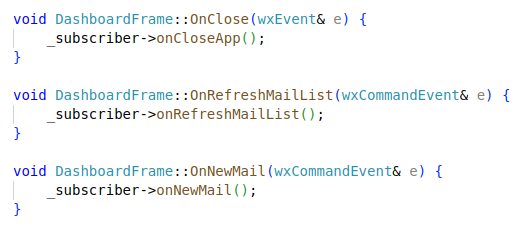
\includegraphics[width=\textwidth]{subscriberFxns.png}
    \caption{Exemple de "event handlers" care apelează funcțiile "subscriber"-ului său, în \texttt{DashboardFrame.cpp}.}
    \label{fig:subscriberFxns}
\end{figure}

\subsubsection{Administrarea conexiunilor POP3 și SMTP.}

Conexiunile cu serverele POP3 și SMTP sunt administrate de clasele POP3Connection și SMTPConnection, care asigură comunicarea corectă cu acestea conform protocoalelor corespunzătoare. 

În general, după o anumită perioadă de inactivitate configurată de către administratorii serverelor, acestea pot încheia conexiunea. O particularitate interesantă a claselor POP3Connection și SMTPConnection este folosirea unui \texttt{std::thread} pentru a menține conexiunile active chiar și după mai mult timp: acesta trimite la un anumit interval repetat de timp, conform protocolului corespunzător, o operație de tip "no-op", prin care să semnaleze activitate fără a realiza o operație propriu-zisă.

În POP3Connection și SMTPConnection există membrul \texttt{\_noopThread} și o metodă \texttt{keepAlive()} care este executată de către acesta. Pentru ca "no-op"-urile trimise de acest thread să nu interfereze cu procesul comandă-răspuns se folosește un \texttt{\_commandMutex}, folosit în funcția \texttt{execCommand} care este apelată atât de comenzi reale, cât și de "no-op". De asemenea, mutexul \texttt{\_stateMutex} este utilizat, printre altele, pentru a actualiza și verifica în mod sigur statusul curent al conexiunii.

\begin{figure}
    \centering
    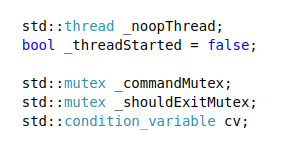
\includegraphics[width={130px}]{noopThread.png}
    \caption{Declararea \texttt{\_noopThread} și a altor membri ajutători în \texttt{POP3Connection.hpp}.}
    \label{fig:noopThread}
\end{figure}

\begin{figure}
    \centering
    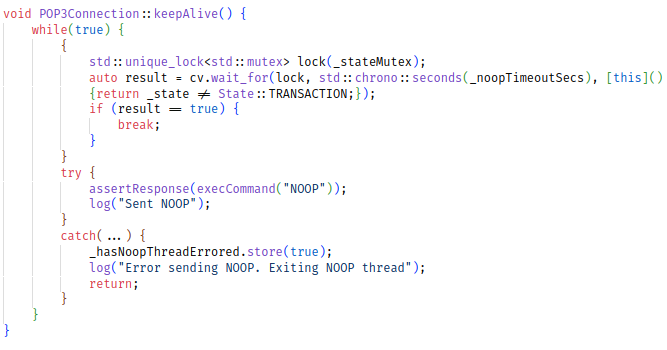
\includegraphics[width=\textwidth]{keepAlive.png}
    \caption{Definiția \texttt{keepAlive()} în \texttt{POP3Connection.cpp}.}
    \label{fig:keepalive}
\end{figure}

\section{Concluzii}

Proiectul funcționează într-un scenariu limitat. Acesta comunică ne-încriptat cu un server POP3 pe \texttt{localhost} cu autentificare bazată pe username și parolă în plain-text, și cu un server SMTP ne-încriptat, fără autentificare, care trimite mailuri doar în rețeaua locală. Din păcate, majoritatea serverelor POP3 și SMTP externe existente astăzi cer un anumit nivel de încriptare a datelor trimise în rețea și de o configurare mai complexă; așadar, practicalitatea proiectului este limitată. Modificarea proiectului pentru a permite comunicarea cu aceste servere nu ar fi imposibilă, dar ar necesita un grad mai mare de complexitate și ar implica dependențe față de mai multe librării externe care să se ocupe de comunicarea securizată în rețea.

De asemenea, librăria wxWidgets are propriile limitări. Fiindcă se bazează pe elemente existente în interfețele sistemelor de operare cu care este compatibilă\cite{ref_wxwidgets}, aceasta nu este la fel de personalizabilă ca unele alternative precum Qt. O posibilă îmbunătățire (dacă se dorește personalizarea mai detaliată a proiectului) ar putea fi portarea la o altă librărie pentru interfața grafică.
%
% ---- Bibliography ----
%
% BibTeX users should specify bibliography style 'splncs04'.
% References will then be sorted and formatted in the correct style.
%
% \bibliographystyle{splncs04}
% \bibliography{mybibliography}

\renewcommand\refname{Referințe bibliografice}
\begin{thebibliography}{8}
\bibitem{ref_rfc_pop3}
RFC 1939, \url{https://www.ietf.org/rfc/rfc1939.txt}. Accesat cel mai recent pe 14 Dec 2023

\bibitem{ref_rfc_smtp}
RFC 5321, \url{https://www.ietf.org/rfc/rfc5321.txt}. Accesat cel mai recent pe 14 Dec 2023

\bibitem{ref_rfc_mime}
RFC 2045, \url{https://datatracker.ietf.org/doc/html/rfc2045}. Accesat cel mai recent pe 14 Dec 2023

\bibitem{ref_wxwidgets}
Pagina principală wxWidgets, \url{https://www.wxwidgets.org/}. Accesat cel mai recent pe 14 Dec 2023


\end{thebibliography}
\end{document}
